% Created by tikzDevice version 0.7.0 on 2016-09-15 08:43:33
% !TEX encoding = UTF-8 Unicode
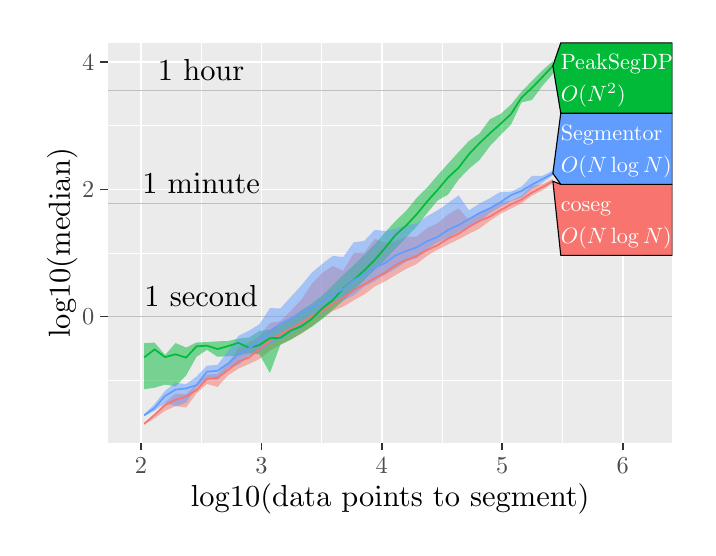
\begin{tikzpicture}[x=1pt,y=1pt]
\definecolor[named]{fillColor}{rgb}{1.00,1.00,1.00}
\path[use as bounding box,fill=fillColor,fill opacity=0.00] (0,0) rectangle (238.49,180.67);
\begin{scope}
\path[clip] (  0.00,  0.00) rectangle (238.49,180.67);
\definecolor[named]{drawColor}{rgb}{1.00,1.00,1.00}
\definecolor[named]{fillColor}{rgb}{1.00,1.00,1.00}

\path[draw=drawColor,line width= 0.6pt,line join=round,line cap=round,fill=fillColor] (  0.00,  0.00) rectangle (238.49,180.68);
\end{scope}
\begin{scope}
\path[clip] ( 29.02, 30.69) rectangle (232.99,175.17);
\definecolor[named]{fillColor}{rgb}{0.92,0.92,0.92}

\path[fill=fillColor] ( 29.02, 30.69) rectangle (232.99,175.18);
\definecolor[named]{drawColor}{rgb}{1.00,1.00,1.00}

\path[draw=drawColor,line width= 0.3pt,line join=round] ( 29.02, 53.31) --
	(232.99, 53.31);

\path[draw=drawColor,line width= 0.3pt,line join=round] ( 29.02, 99.25) --
	(232.99, 99.25);

\path[draw=drawColor,line width= 0.3pt,line join=round] ( 29.02,145.18) --
	(232.99,145.18);

\path[draw=drawColor,line width= 0.3pt,line join=round] ( 62.69, 30.69) --
	( 62.69,175.17);

\path[draw=drawColor,line width= 0.3pt,line join=round] (106.21, 30.69) --
	(106.21,175.17);

\path[draw=drawColor,line width= 0.3pt,line join=round] (149.73, 30.69) --
	(149.73,175.17);

\path[draw=drawColor,line width= 0.3pt,line join=round] (193.25, 30.69) --
	(193.25,175.17);

\path[draw=drawColor,line width= 0.6pt,line join=round] ( 29.02, 76.28) --
	(232.99, 76.28);

\path[draw=drawColor,line width= 0.6pt,line join=round] ( 29.02,122.22) --
	(232.99,122.22);

\path[draw=drawColor,line width= 0.6pt,line join=round] ( 29.02,168.15) --
	(232.99,168.15);

\path[draw=drawColor,line width= 0.6pt,line join=round] ( 40.93, 30.69) --
	( 40.93,175.17);

\path[draw=drawColor,line width= 0.6pt,line join=round] ( 84.45, 30.69) --
	( 84.45,175.17);

\path[draw=drawColor,line width= 0.6pt,line join=round] (127.97, 30.69) --
	(127.97,175.17);

\path[draw=drawColor,line width= 0.6pt,line join=round] (171.49, 30.69) --
	(171.49,175.17);

\path[draw=drawColor,line width= 0.6pt,line join=round] (215.02, 30.69) --
	(215.02,175.17);
\definecolor[named]{drawColor}{rgb}{0.75,0.75,0.75}
\definecolor[named]{fillColor}{rgb}{0.75,0.75,0.75}

\path[draw=drawColor,line width= 0.6pt,line join=round,fill=fillColor] ( 29.02, 76.28) -- (232.99, 76.28);

\path[draw=drawColor,line width= 0.6pt,line join=round,fill=fillColor] ( 29.02,117.12) -- (232.99,117.12);

\path[draw=drawColor,line width= 0.6pt,line join=round,fill=fillColor] ( 29.02,157.96) -- (232.99,157.96);
\definecolor[named]{fillColor}{rgb}{0.97,0.46,0.43}

\path[fill=fillColor,fill opacity=0.50] ( 42.08, 37.74) --
	( 45.87, 40.96) --
	( 49.66, 45.34) --
	( 53.44, 48.38) --
	( 57.23, 48.21) --
	( 61.02, 51.80) --
	( 64.81, 55.29) --
	( 68.59, 55.53) --
	( 72.38, 59.28) --
	( 76.17, 65.00) --
	( 79.96, 66.94) --
	( 83.74, 69.28) --
	( 87.53, 73.93) --
	( 91.32, 74.64) --
	( 95.10, 78.37) --
	( 98.89, 82.35) --
	(102.68, 88.08) --
	(106.47, 92.09) --
	(110.25, 94.50) --
	(114.04, 92.85) --
	(117.83, 99.21) --
	(121.61, 99.40) --
	(125.40,104.33) --
	(129.19,103.00) --
	(132.98,103.48) --
	(136.76,105.16) --
	(140.55,105.18) --
	(144.34,108.28) --
	(148.12,109.99) --
	(151.91,113.17) --
	(155.70,115.39) --
	(159.49,111.10) --
	(163.27,113.68) --
	(167.06,115.64) --
	(170.85,117.58) --
	(174.63,118.21) --
	(178.42,119.98) --
	(182.21,123.67) --
	(186.00,124.11) --
	(189.78,126.04) --
	(189.78,124.44) --
	(186.00,121.94) --
	(182.21,119.99) --
	(178.42,117.17) --
	(174.63,115.30) --
	(170.85,113.39) --
	(167.06,110.94) --
	(163.27,108.08) --
	(159.49,106.22) --
	(155.70,104.19) --
	(151.91,102.35) --
	(148.12,100.48) --
	(144.34, 98.25) --
	(140.55, 95.26) --
	(136.76, 93.51) --
	(132.98, 91.28) --
	(129.19, 89.03) --
	(125.40, 87.14) --
	(121.61, 84.26) --
	(117.83, 82.17) --
	(114.04, 79.87) --
	(110.25, 78.28) --
	(106.47, 75.75) --
	(102.68, 72.72) --
	( 98.89, 70.06) --
	( 95.10, 68.04) --
	( 91.32, 66.14) --
	( 87.53, 63.93) --
	( 83.74, 60.94) --
	( 79.96, 59.12) --
	( 76.17, 57.49) --
	( 72.38, 55.04) --
	( 68.59, 50.83) --
	( 64.81, 51.92) --
	( 61.02, 48.54) --
	( 57.23, 43.39) --
	( 53.44, 43.92) --
	( 49.66, 42.25) --
	( 45.87, 39.48) --
	( 42.08, 37.25) --
	cycle;
\definecolor[named]{fillColor}{rgb}{0.00,0.73,0.22}

\path[fill=fillColor,fill opacity=0.50] ( 42.08, 66.70) --
	( 45.87, 66.86) --
	( 49.66, 62.41) --
	( 53.44, 66.73) --
	( 57.23, 65.07) --
	( 61.02, 66.91) --
	( 64.81, 67.06) --
	( 68.59, 67.34) --
	( 72.38, 67.43) --
	( 76.17, 68.31) --
	( 79.96, 68.68) --
	( 83.74, 71.15) --
	( 87.53, 71.44) --
	( 91.32, 73.01) --
	( 95.10, 75.70) --
	( 98.89, 78.54) --
	(102.68, 80.96) --
	(106.47, 83.87) --
	(110.25, 87.58) --
	(114.04, 91.33) --
	(117.83, 94.84) --
	(121.61, 98.54) --
	(125.40,102.42) --
	(129.19,106.76) --
	(132.98,110.86) --
	(136.76,114.50) --
	(140.55,119.13) --
	(144.34,122.88) --
	(148.12,127.31) --
	(151.91,131.55) --
	(155.70,135.72) --
	(159.49,139.78) --
	(163.27,142.43) --
	(167.06,147.62) --
	(170.85,149.47) --
	(174.63,152.87) --
	(178.42,157.54) --
	(182.21,161.40) --
	(186.00,165.20) --
	(189.78,168.61) --
	(189.78,163.94) --
	(186.00,159.66) --
	(182.21,154.53) --
	(178.42,153.66) --
	(174.63,145.59) --
	(170.85,141.83) --
	(167.06,137.91) --
	(163.27,132.85) --
	(159.49,129.70) --
	(155.70,125.79) --
	(151.91,120.36) --
	(148.12,118.24) --
	(144.34,113.64) --
	(140.55,108.80) --
	(136.76,104.82) --
	(132.98,100.86) --
	(129.19, 96.86) --
	(125.40, 93.13) --
	(121.61, 89.43) --
	(117.83, 85.86) --
	(114.04, 82.09) --
	(110.25, 78.74) --
	(106.47, 75.37) --
	(102.68, 72.61) --
	( 98.89, 70.31) --
	( 95.10, 67.93) --
	( 91.32, 66.09) --
	( 87.53, 55.85) --
	( 83.74, 62.65) --
	( 79.96, 63.03) --
	( 76.17, 62.21) --
	( 72.38, 61.92) --
	( 68.59, 61.75) --
	( 64.81, 64.27) --
	( 61.02, 61.75) --
	( 57.23, 54.96) --
	( 53.44, 51.08) --
	( 49.66, 51.69) --
	( 45.87, 50.57) --
	( 42.08, 50.03) --
	cycle;
\definecolor[named]{fillColor}{rgb}{0.38,0.61,1.00}

\path[fill=fillColor,fill opacity=0.50] ( 42.08, 40.96) --
	( 45.87, 44.66) --
	( 49.66, 49.46) --
	( 53.44, 52.37) --
	( 57.23, 51.80) --
	( 61.02, 54.62) --
	( 64.81, 58.54) --
	( 68.59, 58.83) --
	( 72.38, 63.76) --
	( 76.17, 69.32) --
	( 79.96, 71.15) --
	( 83.74, 73.49) --
	( 87.53, 79.32) --
	( 91.32, 79.23) --
	( 95.10, 83.38) --
	( 98.89, 87.49) --
	(102.68, 92.19) --
	(106.47, 95.33) --
	(110.25, 98.19) --
	(114.04, 97.82) --
	(117.83,103.12) --
	(121.61,103.63) --
	(125.40,107.59) --
	(129.19,107.20) --
	(132.98,107.98) --
	(136.76,109.25) --
	(140.55,109.86) --
	(144.34,112.57) --
	(148.12,114.67) --
	(151.91,117.29) --
	(155.70,120.07) --
	(159.49,114.66) --
	(163.27,117.15) --
	(167.06,119.07) --
	(170.85,121.36) --
	(174.63,121.38) --
	(178.42,123.21) --
	(182.21,127.08) --
	(186.00,127.11) --
	(189.78,129.06) --
	(189.78,127.37) --
	(186.00,124.58) --
	(182.21,122.47) --
	(178.42,119.31) --
	(174.63,117.96) --
	(170.85,115.92) --
	(167.06,113.76) --
	(163.27,110.60) --
	(159.49,108.58) --
	(155.70,106.87) --
	(151.91,104.69) --
	(148.12,103.09) --
	(144.34,100.64) --
	(140.55, 97.35) --
	(136.76, 96.19) --
	(132.98, 93.61) --
	(129.19, 91.45) --
	(125.40, 89.15) --
	(121.61, 87.18) --
	(117.83, 83.99) --
	(114.04, 82.15) --
	(110.25, 80.56) --
	(106.47, 77.48) --
	(102.68, 75.47) --
	( 98.89, 72.06) --
	( 95.10, 70.09) --
	( 91.32, 67.86) --
	( 87.53, 66.14) --
	( 83.74, 63.44) --
	( 79.96, 62.08) --
	( 76.17, 58.83) --
	( 72.38, 57.62) --
	( 68.59, 53.51) --
	( 64.81, 53.60) --
	( 61.02, 50.83) --
	( 57.23, 45.12) --
	( 53.44, 43.92) --
	( 49.66, 45.12) --
	( 45.87, 42.25) --
	( 42.08, 40.25) --
	cycle;
\definecolor[named]{drawColor}{rgb}{0.97,0.46,0.43}

\path[draw=drawColor,line width= 0.6pt,line join=round] ( 42.08, 37.50) --
	( 45.87, 40.79) --
	( 49.66, 44.29) --
	( 53.44, 46.19) --
	( 57.23, 47.35) --
	( 61.02, 49.68) --
	( 64.81, 53.75) --
	( 68.59, 54.12) --
	( 72.38, 56.95) --
	( 76.17, 59.97) --
	( 79.96, 61.46) --
	( 83.74, 64.53) --
	( 87.53, 67.53) --
	( 91.32, 69.86) --
	( 95.10, 71.95) --
	( 98.89, 74.05) --
	(102.68, 76.35) --
	(106.47, 78.31) --
	(110.25, 80.91) --
	(114.04, 83.04) --
	(117.83, 85.84) --
	(121.61, 87.89) --
	(125.40, 90.21) --
	(129.19, 92.15) --
	(132.98, 94.91) --
	(136.76, 96.73) --
	(140.55, 98.18) --
	(144.34,100.33) --
	(148.12,102.05) --
	(151.91,104.47) --
	(155.70,106.19) --
	(159.49,108.71) --
	(163.27,110.81) --
	(167.06,112.43) --
	(170.85,114.73) --
	(174.63,116.79) --
	(178.42,118.51) --
	(182.21,121.07) --
	(186.00,123.04) --
	(189.78,125.19);
\definecolor[named]{drawColor}{rgb}{0.00,0.73,0.22}

\path[draw=drawColor,line width= 0.6pt,line join=round] ( 42.08, 61.51) --
	( 45.87, 64.42) --
	( 49.66, 61.62) --
	( 53.44, 62.65) --
	( 57.23, 61.44) --
	( 61.02, 65.52) --
	( 64.81, 65.76) --
	( 68.59, 64.53) --
	( 72.38, 65.60) --
	( 76.17, 66.78) --
	( 79.96, 64.99) --
	( 83.74, 66.00) --
	( 87.53, 68.47) --
	( 91.32, 68.59) --
	( 95.10, 71.26) --
	( 98.89, 72.73) --
	(102.68, 75.46) --
	(106.47, 79.28) --
	(110.25, 82.22) --
	(114.04, 86.47) --
	(117.83, 89.49) --
	(121.61, 92.95) --
	(125.40, 96.75) --
	(129.19,101.12) --
	(132.98,105.83) --
	(136.76,109.16) --
	(140.55,113.22) --
	(144.34,117.84) --
	(148.12,122.04) --
	(151.91,126.54) --
	(155.70,130.03) --
	(159.49,134.99) --
	(163.27,138.95) --
	(167.06,142.53) --
	(170.85,145.91) --
	(174.63,149.44) --
	(178.42,155.37) --
	(182.21,158.91) --
	(186.00,162.85) --
	(189.78,166.89);
\definecolor[named]{drawColor}{rgb}{0.38,0.61,1.00}

\path[draw=drawColor,line width= 0.6pt,line join=round] ( 42.08, 40.61) --
	( 45.87, 43.26) --
	( 49.66, 47.61) --
	( 53.44, 49.89) --
	( 57.23, 50.31) --
	( 61.02, 51.51) --
	( 64.81, 56.38) --
	( 68.59, 56.67) --
	( 72.38, 59.28) --
	( 76.17, 62.72) --
	( 79.96, 64.71) --
	( 83.74, 67.73) --
	( 87.53, 71.05) --
	( 91.32, 73.66) --
	( 95.10, 75.58) --
	( 98.89, 77.69) --
	(102.68, 79.53) --
	(106.47, 81.83) --
	(110.25, 84.17) --
	(114.04, 86.28) --
	(117.83, 89.33) --
	(121.61, 91.63) --
	(125.40, 93.91) --
	(129.19, 95.65) --
	(132.98, 98.41) --
	(136.76, 99.97) --
	(140.55,101.28) --
	(144.34,103.48) --
	(148.12,105.08) --
	(151.91,107.59) --
	(155.70,109.31) --
	(159.49,111.52) --
	(163.27,113.69) --
	(167.06,115.39) --
	(170.85,117.60) --
	(174.63,120.16) --
	(178.42,121.63) --
	(182.21,123.96) --
	(186.00,125.93) --
	(189.78,128.00);
\definecolor[named]{drawColor}{rgb}{0.00,0.00,0.00}

\node[text=drawColor,anchor=base,inner sep=0pt, outer sep=0pt, scale=  1.10] at ( 62.69, 80.08) {1 second};

\node[text=drawColor,anchor=base,inner sep=0pt, outer sep=0pt, scale=  1.10] at ( 62.69,120.92) {1 minute};

\node[text=drawColor,anchor=base,inner sep=0pt, outer sep=0pt, scale=  1.10] at ( 62.69,161.76) {1 hour};
\end{scope}
\begin{scope}
\path[clip] ( 29.02, 30.69) rectangle (232.99,175.17);
\definecolor[named]{drawColor}{rgb}{0.00,0.00,0.00}
\definecolor[named]{fillColor}{rgb}{0.97,0.46,0.43}

\path[draw=drawColor,line width= 0.4pt,line join=round,line cap=round,fill=fillColor] (189.78,125.19) --
	(192.63,124.06) --
	(232.99,124.06) --
	(232.99, 98.38) --
	(192.63, 98.38) --
	cycle;
\definecolor[named]{fillColor}{rgb}{0.38,0.61,1.00}

\path[draw=drawColor,line width= 0.4pt,line join=round,line cap=round,fill=fillColor] (189.78,128.00) --
	(192.63,149.75) --
	(232.99,149.75) --
	(232.99,124.06) --
	(192.63,124.06) --
	cycle;
\definecolor[named]{fillColor}{rgb}{0.00,0.73,0.22}

\path[draw=drawColor,line width= 0.4pt,line join=round,line cap=round,fill=fillColor] (189.78,166.89) --
	(192.63,175.17) --
	(232.99,175.17) --
	(232.99,149.75) --
	(192.63,149.75) --
	cycle;
\definecolor[named]{drawColor}{rgb}{1.00,1.00,1.00}

\node[text=drawColor,anchor=base west,inner sep=0pt, outer sep=0pt, scale=  0.80] at (192.63,114.24) {coseg};

\node[text=drawColor,anchor=base west,inner sep=0pt, outer sep=0pt, scale=  0.80] at (192.63,102.66) {$O(N \log N)$};

\node[text=drawColor,anchor=base west,inner sep=0pt, outer sep=0pt, scale=  0.80] at (192.63,139.93) {Segmentor};

\node[text=drawColor,anchor=base west,inner sep=0pt, outer sep=0pt, scale=  0.80] at (192.63,128.34) {$O(N \log N)$};

\node[text=drawColor,anchor=base west,inner sep=0pt, outer sep=0pt, scale=  0.80] at (192.63,165.45) {PeakSegDP};

\node[text=drawColor,anchor=base west,inner sep=0pt, outer sep=0pt, scale=  0.80] at (192.63,153.98) {$O(N^2)$};
\end{scope}
\begin{scope}
\path[clip] (  0.00,  0.00) rectangle (238.49,180.67);
\definecolor[named]{drawColor}{rgb}{0.30,0.30,0.30}

\node[text=drawColor,anchor=base east,inner sep=0pt, outer sep=0pt, scale=  0.88] at ( 24.07, 73.25) {0};

\node[text=drawColor,anchor=base east,inner sep=0pt, outer sep=0pt, scale=  0.88] at ( 24.07,119.19) {2};

\node[text=drawColor,anchor=base east,inner sep=0pt, outer sep=0pt, scale=  0.88] at ( 24.07,165.12) {4};
\end{scope}
\begin{scope}
\path[clip] (  0.00,  0.00) rectangle (238.49,180.67);
\definecolor[named]{drawColor}{rgb}{0.20,0.20,0.20}

\path[draw=drawColor,line width= 0.6pt,line join=round] ( 26.27, 76.28) --
	( 29.02, 76.28);

\path[draw=drawColor,line width= 0.6pt,line join=round] ( 26.27,122.22) --
	( 29.02,122.22);

\path[draw=drawColor,line width= 0.6pt,line join=round] ( 26.27,168.15) --
	( 29.02,168.15);
\end{scope}
\begin{scope}
\path[clip] (  0.00,  0.00) rectangle (238.49,180.67);
\definecolor[named]{drawColor}{rgb}{0.20,0.20,0.20}

\path[draw=drawColor,line width= 0.6pt,line join=round] ( 40.93, 27.94) --
	( 40.93, 30.69);

\path[draw=drawColor,line width= 0.6pt,line join=round] ( 84.45, 27.94) --
	( 84.45, 30.69);

\path[draw=drawColor,line width= 0.6pt,line join=round] (127.97, 27.94) --
	(127.97, 30.69);

\path[draw=drawColor,line width= 0.6pt,line join=round] (171.49, 27.94) --
	(171.49, 30.69);

\path[draw=drawColor,line width= 0.6pt,line join=round] (215.02, 27.94) --
	(215.02, 30.69);
\end{scope}
\begin{scope}
\path[clip] (  0.00,  0.00) rectangle (238.49,180.67);
\definecolor[named]{drawColor}{rgb}{0.30,0.30,0.30}

\node[text=drawColor,anchor=base,inner sep=0pt, outer sep=0pt, scale=  0.88] at ( 40.93, 19.68) {2};

\node[text=drawColor,anchor=base,inner sep=0pt, outer sep=0pt, scale=  0.88] at ( 84.45, 19.68) {3};

\node[text=drawColor,anchor=base,inner sep=0pt, outer sep=0pt, scale=  0.88] at (127.97, 19.68) {4};

\node[text=drawColor,anchor=base,inner sep=0pt, outer sep=0pt, scale=  0.88] at (171.49, 19.68) {5};

\node[text=drawColor,anchor=base,inner sep=0pt, outer sep=0pt, scale=  0.88] at (215.02, 19.68) {6};
\end{scope}
\begin{scope}
\path[clip] (  0.00,  0.00) rectangle (238.49,180.67);
\definecolor[named]{drawColor}{rgb}{0.00,0.00,0.00}

\node[text=drawColor,anchor=base,inner sep=0pt, outer sep=0pt, scale=  1.10] at (131.01,  7.70) {log10(data points to segment)};
\end{scope}
\begin{scope}
\path[clip] (  0.00,  0.00) rectangle (238.49,180.67);
\definecolor[named]{drawColor}{rgb}{0.00,0.00,0.00}

\node[text=drawColor,rotate= 90.00,anchor=base,inner sep=0pt, outer sep=0pt, scale=  1.10] at ( 15.28,102.93) {log10(median)};
\end{scope}
\end{tikzpicture}
